\documentclass[leqno, 12pt]{book}

\usepackage{mystyle, subfiles}
\usepackage{wasysym, glossaries, nomencl}
%\usepackage{times, mathptmx}
%Print the pages you want!
\usepackage[1-13, 229-351]{pagesel}

\title{\bf\Huge	\colorbox{black!30}{TOPICS IN NUMBER THEORY:}\\ \it \Large \colorbox{black!30}{An Olympiad-Oriented Approach}}
\author{	\Large
	\it \bf \colorbox{black!30}{Masum Billal}%\\University of Dhaka\\Dhaka, Bangladesh\\
	%Email: \href{mailto:billalmasum93@gmail.com}{billalmasum93@gmail.com}
	\and \Large
	\it \bf \colorbox{black!30}{Amir Hossein Parvardi}%\\University of Tehran\\Tehran, Iran\\
	%Email: \href{mailto:a.parvardi@gmail.com}{a.parvardi@gmail.com}
}
\date{\Huge \bf \colorbox{black!20}{Sample Chapters}\\\colorbox{black!20}{Version 1.1.}\\\colorbox{black!20}{July 2018}}


\DeclareUnicodeCharacter{2212}{-}

%\makenomenclature
%\renewcommand{\nomname}{Notations}

%% Riemann's paper in the background, of course:
\usepackage{eso-pic}
\newcommand\BackgroundPic{%
	\put(0,0){%
		\parbox[b][\paperheight]{\paperwidth}{%
			\vfill
			\centering
			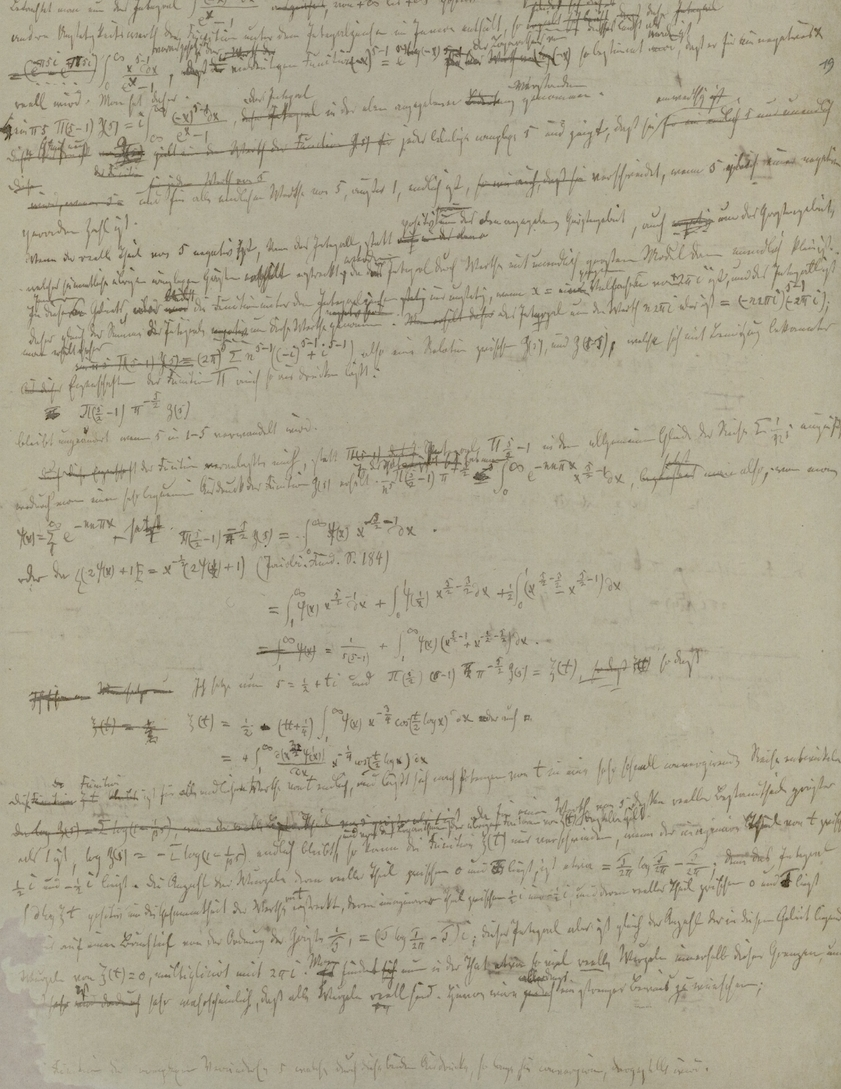
\includegraphics[width=\paperwidth,height=\paperheight,%
			keepaspectratio]{background.jpg}%
			\vfill
}}}

\begin{document}
\AddToShipoutPicture*{\BackgroundPic}

\pagenumbering{arabic}
\frontmatter
\maketitle
\pagestyle{plain}
\pagenumbering{arabic}
\setcounter{page}{2}
\begin{dedication}
	%\begin{center}
	%	\textbf{Editing Acknowledgment}
	%\end{center}
	%{\slshape Nur Muhammad Shafiullah (also known as Hojor Shofi, first of his name, hojor of the BdMO camp, murid of the hojormaker, sophomore at MIT, job holder at some company)}, for his valuable editions and suggestions that made this book better.
	\begin{center}
		\textbf{Dedicated to}
	\end{center}\slshape
	Our regular studies, without which, we could have finished this book long time ago.\\
	Fermat, the father of modern number theory.\\
	Euler, without whom number theory probably wouldn't be so rich today.\\
	Ramanujan, mathematician of mathematicians.\\
	Paul Erd\H{o}s, the man who loved only numbers.
\end{dedication}

\section*{Links}

\begin{itemize}
	\item The website of the book always contains the updates, errata, and new free materials that we regularly post on social media. Exclusive olympiad problem-sets will be released in the website in the near fuure: \begin{center}
		\url{https:/TopicsInNumberTheory.com}
	\end{center}

	\item Facebook page:
		\begin{center}
			\url{https://facebook.com/TopicsInNumberTheory/}
		\end{center}
	This is our main page for feedback and reviews on the book. Feel free to post any kind of review, comment, solution, or suggestion you have about this book. Amir Hossein will create a forum for the book on AoPS so everyone can post their solutions to be added to the book later on.
	\item If you find any mistake or typo in the book, we would be happy to hear it at Facebook or \href{mailto:info@TopicsInNumberTheory.com}{info@TopicsInNumberTheory.com}.
	
	\item This is version 1.1. of the sample chapters, including chapters 4 (Primes) and 5 (Special Topics) plus the appendix. As we update the book, we also update these samples also on our website. To keep track of the latest updates, please keep this URL (from which you downloaded the file) somewhere safe:
		\begin{center}
			\url{https://TopicsInNumberTheory.com/download/samplechapters/}
		\end{center}
	The password might be changed for the future updates, but we will always send the new passwords to our subscribers in Facebook and in the newsletter.
	\item The password for this edition is \texttt{Riemann}.
\end{itemize}

\section*{Copyright Notice}
The cover shows a part of the famous paper of Bernhard Riemann in 1859 in Number Theory. It was taken from the website of Clay Mathematics Institute. You can read \href{http://www.claymath.org/sites/default/files/riemann1859.pdf}{the original manuscript} as well as the \href{http://www.claymath.org/sites/default/files/ezeta.pdf}{English translation} of this wonderful paper by David Wilkins in their website:
	\begin{center}
			\url{http://www.claymath.org/publications/riemanns-1859-manuscript}
	\end{center}



This file was prepared by Masum Billal and Amir Hossein Parvardi, as a gift to all the kind people who were looking forward to reading our book. You can read this PDF, print the file on paper, share it with your friends, or discuss the problems on our Facebook page, but please do not upload this PDF file into the public. Keep it private! 
\vspace{0.3cm}
\begin{center}
Copyright $^{\tiny{\textcopyright}}$ 2018 TopicsInNumberTheory.com\\
Masum Billal and Amir Hossein Parvardi\\
All rights reserved.


\end{center}

\newpage
\section*{First Words by Masum}
%	We would like to have a few words before diving into the discussion. First of all, from
%	our personal experience, we have found that there is a common practice to learn by
%	learning a lot of theories and then investigating how those theories are used to solve
%	problems. As our primary audience would be students who are looking to get into
%	mathematical olympiads, we highly discourage this. Please do not take number theory
%	for a collection of theories just because there is literally the word theory in it.
%	That being said, one could say that our book itself is a collection of a lot of theorems
%	as well. Sadly, that is partially true for multiple reasons even though it was not our
%	intention at all.
%	When we first thought about writing this book, our intention was to make students
%	realize that they do not need to know a lot of theories in order to have an idea about
%	number theory. Our target was to show solutions to problems without using much
%	theory, or at least in a manner that gives them an idea of how a problem could be
%	solved even if they did not have any idea about that theory. But as we kept writing we had
%	to increase the pace since we had to cover a lot (and that was after discarding a lot
%	of contents which we thought would ask for even more discussion or we just felt lazy
%	about it), we had to increase the pace.
%	
%	We would like to address one more concern. Originally, our plan was to make this book a series of $5$ volumes, this being the first one. In those volumes we wanted to discuss a lot of topics such as special numbers like \textit{egyptian fraction} or even interesting numbers like \textit{abundant number or deficient number} and their properties etc or crucial topics such as \textit{Diophantine equations}. You will notice that we have left a lot of important topics like those out of this book. The reason is, we quickly realized we can hardly finish writing this one, and if we wanted to complete the series we will probably have to keep writing our whole life. So, we had to discard a lot of contents and make the book concise which resulted in squeezing in a lot of contents in a few hundreds of pages. We would be satisfied if we could actually finish what we planned. Maybe we will someday, but at the moment, we have neither the time nor the energy to do so.
%		\begin{flushright}
%			\sl Masum Billal\\
%			July 2018.
%		\end{flushright}

%I would like to have a few words before diving into the discussion. First of all, from my personal experience, I have found that there is a common practice to learn1 by learning a lot of theories and then investigating how those theories are used to solve problems. As our primary audience would be students who are looking to get into mathematical olympiads, I highly discourage this. Please do not take number theory for a collection of theories just because the word theory is literally juxtaposed with it. That being said, one could say that our book itself is a collection of a lot of theorems as well. Sadly, that is partially true for multiple reasons even though it was not our intention at all.
%
%
%\vspace{0.3cm}
%
%When I first thought about writing this book, my intention was to make students realize that they do not need to know a lot of theorems in order to be able to solve problems. My primary target was to build confidence about this claim. But as we kept writing we had to increase the pace since we had to cover a lot (and that was  discarding a lot of contents which we thought would ask for even discussion or we just felt lazy about it), we had to increase the pace.
%
%
%\vspace{0.3cm}
%
%Probably I should warn the readers to not use this book as a reference or first text book when it comes to formal definitions or rigorous stuff like that. You can still use it for theorems but you may find lack of rigorousness. The reason is that one of my goals was to not be entirely rigorous and formal with the definitions or approaches. Rather I wanted to write in a way that would make better sense, like what made me approach this way and why it could have been solved without knowing a particular theorem. For that, I have got objections from a few people but I followed my own style anyway. In cases, some people may even argue that the book is not very professional or inconsistent. For example, we have discussed logarithm whereas we have not discussed function or a lot of other basic topics. This was almost inevitable. We had to cut off many topics like this in order to make room for others, and also at that point we felt like, if someone has become used to reading the book so far, they should have no trouble understanding or learning basics.
%
%
%\vspace{0.3cm}
%
%I would like to address one more concern. Originally, my plan was to make this book a series of $5$ volumes, this being the first one. In those volumes I wanted to discuss a lot of topics such as special numbers like \textit{egyptian fraction} or even interesting numbers like \textit{abundant number or deficient number} and their properties etc or crucial topics such as \textit{Diophantine equations}. You will notice that we have left a lot of important topics like those out of this book. The reason is, I quickly realized I can hardly finish writing this first volume, and if I wanted to complete the series we will probably have to keep writing my whole life. So, I had to discard a lot of contents and make the book concise which resulted in squeezing in a lot of contents in a few hundreds of pages. Finally, I would like to thank Amir to join me in this project. At one point I almost stopped writing the book. If he had not agreed to be a co-author, this book would have probably not been published at all. More so because he agreed to follow the style I wanted to write in even when we had objection from publisher like \textit{Springer}.
%
%\begin{flushright}
%
%	\sl Masum Billal,\\
%
%	Dhaka, Bangladesh,\\
%	July 2018.
%\end{flushright}


	I would like to have a few words before diving into the discussion. First of all, from my personal experience, I have found that there is a common practice to learn1 by learning a lot of theories and then investigating how those theories are used to solve problems. As our primary audience would be students who are looking to get into mathematical olympiads, I highly discourage this. Please do not take number theory for a collection of theories just because the word theory is literally juxtaposed with it. That being said, one could say that our book itself is a collection of a lot of theorems as well. Sadly, that is partially true for multiple reasons even though it was not our intention at all.


When I first thought about writing this book, my intention was to make students realize that they do not need to know a lot of theorems in order to be able to solve problems. My primary target was to build confidence about this claim. But as we kept writing we had to increase the pace since we had to cover a lot (and that was  discarding a lot of contents which we thought would ask for even discussion or we just felt lazy about it), we had to increase the pace.


I would like to address one more concern. Originally, my plan was to make this book a series of $5$ volumes, this being the first one. In those volumes I wanted to discuss a lot of topics such as special numbers like \textit{egyptian fraction} or even interesting numbers like \textit{abundant number or deficient number} and their properties etc or crucial topics such as \textit{Diophantine equations}. You will notice that we have left a lot of important topics like those out of this book. The reason is, I quickly realized I can hardly finish writing this first volume, and if I wanted to complete the series we will probably have to keep writing my whole life. So, I had to discard a lot of contents and make the book concise which resulted in squeezing in a lot of contents in a few hundreds of pages. 


Finally, I would like to thank Amir to join me in this project. At one point I stopped writing the book. If he had not agreed to be a co-author, this book would have probably not been completed at all. More so because he agreed to follow the style I wanted to write in even when we had objection from reputed publisher like \textit{Springer}.

\begin{flushright}

	\sl Masum Billal\\

	July 2018.
\end{flushright}
	
	\newpage
	
\section*{First Words by Amir Hossein}
	In the past three years, we have been always worried about this book. It's been a long and tedious job to manage everything and edit all we had written a very long time ago. After I studied higher level number theory concepts, there were times that I found errors/typos in my previous drafts for the book. And that sometimes happened two or more times in a short period, and so, it was getting annoying. Anyhow, we managed to finish it at this time of the summer. It is now 5:36 AM, Tuesday, July 17, 2018 that I'm writing this. You can imagine how crazy this process has made me!
	
	\vspace{0.3cm}
	
	\textbf{BUT!} a wise man once said ``high quality math books are written in a series of editions in long term,'' and we are happy to hear that. Many of our friends helped us during the way to finish this book, as mentioned in the Acknowledgement, and we are so proud to have such friends.
	
	\vspace{0.3cm}
	
	I wouldn't be able to finish my part in this book if I didn't have the support of my wonderful, beautiful, and lovely wife \textbf{Nadia Ghobadipasha}. She gave me hope to choose mathematics and always believed in me. She was my only one in the hardest days of life.
	
	\vspace{0.3cm}
	
	Professor \textbf{Peyman Nasehpour}, whom I knew from the very first semester of my undergraduate studies in elelctrical englineering at University of Tehran, helped me a lot in the process of enhancing my mathematical abilities to change my field to mathematics (number theory) for my master's.  He is an inspiration to me, and a great colleague when it comes to teamwork. I'm looking forward to working with him more ofter.
	
	\vspace{0.3cm}
	
	The idea behind the lattices in the (paperback) \textbf{cover} is a geometric proof of law of quadratic reciprocity. Our friends found other interpretations of it such as Pick's theorem (which is not the case here) or the sum of positive integers up to $n$, which you will realize is also not always true (for all primes $p,q$). Section \eqref{sec:qrlawproof} is dedicated to this proof and investigates why it is true using counting the lattice (grid) points. When we picked this idea for the cover, we chose quadratic reciprocity because its proof is geometrically visual and indeed very beautiful. Our hope was to make the reader curious because the design looks familiar. Stay excited until you read that proof! Or, maybe, go read it if you have the prerequisite knowledge and the puzzle is boggling your mind. I remember I found the idea of the proof in one of Kenneth H. Rosen's books on discrete mathematics, but I'm not sure which one, as it was a long time ago when I wrote it. I used TikZ package for \LaTeX to write the codes and generate the graphs. 
	
	\vspace{0.3cm}
	
	There are so many wonderful things to learn in this book. I hope you enjoy it!
		\begin{flushright}
		\sl Amir Hossein Parvardi,\\
		University of British Columbia,\\
		Vancouver, BC, Canada,\\
		July 2018.
	\end{flushright}
	
	
	\newpage
\section*{Acknowledgement}

Here is a list of all the kind people who helped us review, edit, and improve this book. We could not decide who to thank more, hence an alphabetically (last name) ordered list:
	\begin{enumerate}
		\item Thanks to \textbf{Ali Amiri}, a kind friend who helped us in the cover design. 
		\item Thanks to \textbf{Anr\' eC} from TeX.StackExchange who wrote the code for figure \eqref{fig:base16} in base conversion.
		\item Thanks to \textbf{Kave Eskandari} for reading the whole book and commenting on the general points. He caught a good mistake in chapter \ref{ch:divisibility}.
		\item Cheers to our mathematical friend \textbf{Leonard Mihai C. Giugiuc} from Romania who gave us positive and constructive feedback on the book. He also wrote us a wonderful review in the website. 

		\item Thanks to \textbf{Valentio Iverson} for proof-reading chapters \ref{ch:arithfunc} and \ref{ch:special}, and pointing out the typo in figure \eqref{fig:unitfunction}.

		\item Thanks to \textbf{Aditya Khurmi} for reading the book and giving us positive feedback.
				
				
		\item We appreciate \textbf{Hesam Korki}'s comments on chapter \ref{ch:divisibility}. He mentioned a few very important typos, including grammatical. He also mentioned a mathematical change in that chapter, which was very helpful.
		
		\item We appreciate \textbf{Kenji Nakagawa}'s precise points on chapters 4 and 5 that we sent to our website subscribers as samples of the book. He sent us a review a few hours after we sent the sample chapters! We are thankful for his quick and useful review.
		
		\item Professor \textbf{Peyman Nasehpour} sent us the beautiful problem \eqref{prob:nasehpour} and an amazing solution using Prime Number Theorem. He also gave us pretty useful comments on chapter \ref{ch:divisibility}. He also introduced in section \eqref{sec:sum-of-divisors} the amicable numbers to us with a brief historical note on it.
				
		\item We are thankful to \textbf{Mohammadamin Nejatbakhshesfahani}, Iran National Olympiad Gold Medalist (2010) and winner of gold medals at IMS and IMC, who honored us toread and reviewe the whole book and gave us really instructive comments.
				
		\item We would like to thank \textbf{Nur Muhammad Shafiullah Mahi} for his efforts to make this book better.
		
		\item We are honored to thank Professor \textbf{Greg Martin}, a faculty member at the Mathematics Department of University of British Columbia. He happens to be Amir Hossein's Master's supervisor. He kindly reviewed a printed draft of the book and emailed us over 10 major points to correct in the book. We do appreciate his advice on improving the whole context of the book.
		
		\item We are thankful to \textbf{Sohrab Mohtat} for his comments on chapter \ref{ch:divisibility}. Thanks to him, we avoided a fatal mistake in the beginning of the book. He also wrote a very useful and detailed review for our book in the website.


		\item We are thankful to \textbf{Aditya Guha Roy} who reviewed the whole book and caught a few LaTeX typos, generalized lemma \eqref{lem:aditya-generalized}, fixing problems in chapter \ref{ch:unsolved}. Aditya wrote an amazing, educative review in our website.
		\item \textbf{Navneel Singhal} carefully reviewed and proof-read the whole first part of the book (chapters \ref{ch:divisibility} to \ref{ch:special}) and gave us very constructive comments. We are thankful to him.
				
		\item Thanks to \textbf{Amin Soofiani}, who is a Master's student of mathematics at University of British Columbia, we noticed there was a mistake in theorem \eqref{thm:numofprime}. He did a perfect, precise, and detailed review on chapter \ref{ch:primes}. 
		




		
		\item We are thankful to \textbf{Sepehr Yadegarzadeh} for informing us about the correct \textit{umlaut}\footnote{\textit{umlaut}: a mark (\"{}) used over a vowel, as in German or Hungarian, to indicate a different vowel quality, usually fronting or rounding.} for M\"{o}bius among other grammatical and vocabulary points.
	\end{enumerate}
	
	\dominitoc
	
\tableofcontents


\pagestyle{myfancy}
\pagestyle{fancy}

\mainmatter

\setcounter{page}{13}

	\section*{Notations}
	\subfile{intro.tex}
\part{Theory and Practice}
	\chapter{Divisibility}\label{ch:divisibility}
	\minitoc \mtcskip \minilof
		\subfile{divisibility.tex}
	\chapter{Modular Arithmetic}\label{ch:congruence}
	\minitoc \mtcskip \minilof
		\subfile{congruence.tex}
	\chapter{Arithmetic Functions}\label{ch:arithfunc}
	 \minitoc \mtcskip \minilof
		\subfile{arithfunc.tex}
	\chapter{Primes}\label{ch:primes}
	\minitoc \mtcskip \minilof
		\subfile{primes.tex}
	\chapter{Special Topics}\label{ch:special}
	\minitoc \mtcskip \minilof
		\subfile{special.tex}
	\begin{appendix}\label{ch:appendices}
		\appendixpage
		\noappendicestocpagenum
		\addappheadtotoc
		%\chapter{Common Identities and Theorems}\label{ch:idthm}
		\chapter{Identities and Well-Known Theorems}\label{ch:null}
			\subfile{idthm.tex}
	\end{appendix}
	\resumechapters	
\part{Problem Column}
	\chapter{Solving Challenge Problems}\label{ch:solved}
		\subfile{solved.tex}
	\chapter{Practice Challenge Problems}\label{ch:unsolved}
		\subfile{unsolved.tex}
		\subfile{unsolved2016.tex}


\end{document}